\documentclass{beamer}
\usetheme{Madrid}

\usepackage{amsmath, amssymb, amsthm}
\usepackage{graphicx}
\usepackage{listings}
\usepackage{gensymb}
\usepackage{minted}
\usemintedstyle{friendly}
\definecolor{bg}{rgb}{1.0, 1.0, 0.8}
\usepackage[utf8]{inputenc}
\usepackage{hyperref}
\usepackage{gvv}
\begin{document}
\title{SOLUTION OF DIFFERENTIAL EQUATION}
\author{EE24BTECH11008 - ASLIN GARVASIS}
\date{}
\frame{\titlepage}

\begin{frame}
\frametitle{Question}
Solve the following second-order nonlinear differential equation:
\begin{equation}
y'' + y'^2 + 2y = 0
\end{equation}
  \end{frame}
  \begin{frame}{allowframebreaks}
\frametitle{Solution}
Finding an exact analytical solution for this nonlinear differential equation is challenging. Hence, we will use the numerical Euler method to obtain an approximate solution.

To apply Euler’s method, we first need to transform the second-order equation into a system of first-order equations.\\
Let
\begin{align}
u &= y'\\
\therefore u' &= y''
\end{align}
\end{frame}
\begin{frame}{Solution}
   Substituting \( y' = u \) into the original equation gives:
\begin{equation}
u' + u^2 + 2y = 0
\end{equation}
This results in the following system of first-order differential equations:
\begin{align}
\frac{dy}{dx} &= u \\
u' =\frac{du}{dx} &= -u^2 - 2y
\end{align}

\end{frame}
\begin{frame}{Euler's Method}
Euler's method approximates the solution of a system of first-order differential equations by updating the solution iteratively. The update rules are given by:
\begin{align}
u'_{n} &= -(u_n)^2 - 2y_n \\	
y_{n+1} &= y_n + h \cdot u_n \\
u_{n+1} &= u_n + h \cdot (u'_n) \\
x_{n+1} &= x_n + h 
\end{align}

Where:
- \( y_n \) ,\( u_n \) and \( u'_n \) are the values of \( y \) ,\( u \) and \( u' \) at the \( n \)-th step.
- \( h \) is the step size that controls the accuracy of the method.
- \( y_{n+1} \) and \( u_{n+1} \) are the updated values at the next step.


\end{frame}
\begin{frame}
\frametitle{Plot}
\begin{figure}
    \centering
    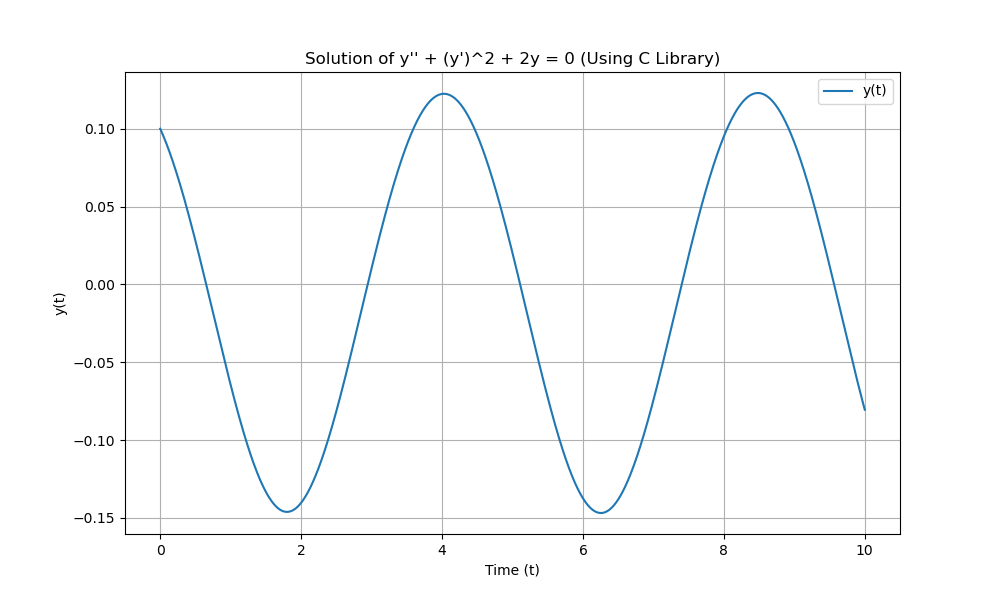
\includegraphics[width=0.7\linewidth]{Fig 9.1.9.png}
\end{figure}
\end{frame}
\begin{frame}[fragile]
\frametitle{C-code}
\begin{minted}[bgcolor=bg, linenos, fontsize=\small, breaklines]{c}
    #include <stdio.h>
#include <stdlib.h>

void solve_ode(double y0, double y_prime0, double dt, double t_max, double* t_values, double* y_values, int size) {
    // Initialize variables
    y_values[0] = y0;
    double y_prime = y_prime0;

    // Numerical integration using Euler's method
    for (int i = 1; i < size; i++) {
        double t = t_values[i - 1];
        double y = y_values[i - 1];
        double y_double_prime = -(y_prime * y_prime) - 2 * y;

       

 \end{minted}   
 \end{frame}
 \begin{frame}[fragile]
 \frametitle{C-code}
   \begin{minted}[bgcolor=bg, linenos, fontsize=\small, breaklines]{c}  
     // Update y and y'
        double y_new = y + y_prime * dt;
        y_prime = y_prime + y_double_prime * dt;

        // Store result
        y_values[i] = y_new;
    }
}
\end{minted}
\end{frame}

\begin{frame}[fragile]
\frametitle{Python code}
    \begin{minted}[bgcolor=bg, linenos, fontsize=\small, breaklines]{python}
import numpy as np
import matplotlib.pyplot as plt
from ctypes import CDLL, POINTER, c_double, c_int

# Load the shared C library that contains the ODE solver function
ode_solver = CDLL("./ode_solver.so")

# Define initial conditions and parameters
y0 = 0.1      # Initial value of the dependent variable y(x)
y_prime0 = -0.1  # Initial value of the first derivative of y, i.e., y'(x)
x_max = 10    # The maximum value of the independent variable (x) (end of range)
dx = 0.001    # The step size for the independent variable (x)

\end{minted}
\end{frame}
\begin{frame}[fragile]
\frametitle{Python code}
\begin{minted}[bgcolor=bg, linenos, fontsize=\small, breaklines]{python}
# Define the number of steps to compute based on the range and step size
num_steps = int(x_max / dx) + 1

# Create an array to store the computed values of y(x) at each step
y_values = np.zeros(num_steps, dtype=np.float64)

# Prepare the input arguments for the C function
x_values_ctypes = np.arange(0, x_max + dx, dx).ctypes.data_as(POINTER(c_double))
y_values_ctypes = y_values.ctypes.data_as(POINTER(c_double))

# Call the ODE solver function from the C library to compute the solution

\end{minted}
\end{frame}

\begin{frame}[fragile]
\frametitle{Python code}
\begin{minted}[bgcolor=bg, linenos, fontsize=\small, breaklines]{python}
# The function signature is expected to accept initial conditions, step size, range, and arrays for independent variable (x) and solution (y)
ode_solver.solve_ode(c_double(y0), c_double(y_prime0), c_double(dx), c_double(x_max), x_values_ctypes, y_values_ctypes, c_int(num_steps))

# Plot the results of the ODE solution
plt.figure(figsize=(10, 6))
plt.plot(np.arange(0, x_max + dx, dx), y_values, label="y(x)")
plt.title("Numerical Solution of a Differential Equation Using C Library")
plt.xlabel("x")
plt.ylabel("y(x)")
plt.grid()
plt.legend()
plt.show()

\end{minted}
\end{frame}

\end{document}
